\documentclass[a4paper]{ltxdoc}

\usepackage[UTF8]{ctex}
\usepackage{unicode-math}
\usepackage{caption}
\usepackage{booktabs}
\usepackage{xcolor}
\usepackage{listings}
\usepackage[perpage]{footmisc}
\usepackage{hypdoc}
\usepackage{amsfonts}
\usepackage{amsmath}
\usepackage{float}
\usepackage{graphicx}

\usepackage{geometry}
\geometry{left=3.3cm, right=3.3cm, top=2.5cm, bottom=3.0cm}

\usepackage{color}

\makeatletter

% 设置字体
\IfFileExists{/System/Library/Fonts/Times.ttc}{
  \setmainfont{Times}
  \setsansfont[Scale=MatchLowercase]{Helvetica}
  \setmonofont[Scale=MatchLowercase]{Menlo}
  \xeCJKsetwidth{‘’“”}{1em}
}{}
\unimathsetup{
  math-style=ISO,
  bold-style=ISO,
}
\IfFontExistsTF{xits-math.otf}{
  \setmathfont[
    Extension    = .otf,
    BoldFont     = *bold,
    StylisticSet = 8,
  ]{xits-math}
  \setmathfont[range={cal,bfcal},StylisticSet=1]{xits-math.otf}
}{
  \setmathfont[
    Extension    = .otf,
    BoldFont     = XITSMath-Bold,
    StylisticSet = 8,
  ]{XITSMath-Regular}
  \setmathfont[range={cal,bfcal},StylisticSet=1]{XITSMath-Regular.otf}
}

% 定义一些命令用于写文档
\newcommand\TeXLive{\TeX{} Live}
\newcommand\unicodechar[1]{U+#1(\symbol{"#1})}
\DeclareRobustCommand\file{\nolinkurl}
\DeclareRobustCommand\env{\texttt}
\DeclareRobustCommand\pkg{\textsf}
\DeclareRobustCommand\cls{\textsf}
\DeclareRobustCommand\opt{\texttt}

% 在 doc 的基础上增加 option 的描述
\def\DescribeOption{\leavevmode\@bsphack\begingroup\MakePrivateLetters
  \Describe@Option}
\def\Describe@Option#1{\endgroup
              \marginpar{\raggedleft\PrintDescribeOption{#1}}%
              \SpecialEnvIndex{#1}\@esphack\ignorespaces}
\@ifundefined{PrintDescribeOption}
   {\def\PrintDescribeOption#1{\strut \MacroFont #1\ }}{}

% 调整列表的格式
\setlength\partopsep{\z@}
\def\@listi{\leftmargin\leftmargini
            \parsep \z@
            \topsep \z@
            \itemsep \z@}
\let\@listI\@listi
\@listi

% listings 的样式
\lstdefinestyle{lstshell}{
  basicstyle      = \small\ttfamily,
  backgroundcolor = \color{lightgray},
  language        = bash,
}
\newcommand\shellcmd[1]{\colorbox{lightgray}{\lstinline[style=lstshell]|#1|}}
\lstnewenvironment{shell}{\lstset{style=lstshell, gobble=2}}{}
\lstnewenvironment{latex}{%
  \lstset{
    basicstyle = \small\ttfamily,
    frame      = single,
    gobble     = 2,
    language   = [LaTeX]TeX,
  }%
}{}

\hypersetup{
  allcolors         = blue,
  bookmarksnumbered = true,
  bookmarksopen     = true,
}
\makeatother


\begin{document}



\title{Matlab-2}
\author{高悟恒 }
\date{\qquad 2020-10-2}
\maketitle



一.问题描述:
在图像编辑中的一个常见问题是将一张图片中的物体放入另一张图片中,但是由于图片背景图案并不一样,直接复制粘贴像素值会导致物体显得比较突兀。其本质问题在于边界点附近的像素值
不连续,而现实生活中总是连续的。先设有一物体图像对应光滑函数$g$,一目标背景图片对应光滑函数$f^*$,现求一函数$f$使得其在边界处与$f^*$相近,同时与$g$有相似特征。




二.算法:
设$\Omega$为物体图像中我们关心的物体对应的定义域点集,$S$为物体图像定义域,对于$S$中任一一点$p$,记$N_p$为其相邻的四个点组成的集合。记$\Omega$的边界为$\partial \Omega=\{p\in S\setminus \Omega:N_p\cap \Omega \neq \emptyset \}$。\\
因此有边界方程:$f\mid_{\partial \Omega}=f^*\mid_{\partial \Omega}$\\
而$f$与对应梯度场与向量成$v$相似,也就是需要求解:
\begin{equation}
\min\limits_f\int\int_{\Omega}\vert\nabla f-v\vert^2,with f\mid_{\partial \Omega}=f^*\mid_{\partial \Omega}
\end{equation}
其与Dirichlet问题的Poisson方程等价,对应离散形式为:
\begin{equation}
\min\limits_{f\mid \Omega}\sum_{<p,q>\cap \Omega\neq \emptyset }(f_p-f_q-v_{pq})^2,with f\mid_{\partial \Omega}=f^*\mid_{\partial \Omega}
\end{equation}
它的解满足下列线性方程组:
\begin{equation}
\vert N_p\vert f_p-\sum_{q\in N_p\cap \Omega}f_q=\sum_{q\in N_p\cap \partial\Omega}f^*_q+\sum_{q\in N_p}v_{pq}
\end{equation}
由此我们得到了一个稀疏线性系统$Ax=b$,由上式显然有$A$为对称正定矩阵,且对于不同的背景$f^*$,$A$是定值,因此可以用Cholesky分解对$A$作预分解,再对不同的$b$求解方程以减少运行时间,达到实时的效果。\\
对于向量场$v$,我们选取混合梯度,即取:
\begin{equation}
v_{pq}=
\begin{cases}
f^*_p-f^*_q&\mbox{if $\vert f^*_p-f^*_q\vert > \vert g_p-g_q\vert$ }\\
g_p-g_q&\mbox{otherwise}
\end{cases}
\end{equation}


\newpage
三.实验结果:
\begin{figure}[htb]
  \centering
  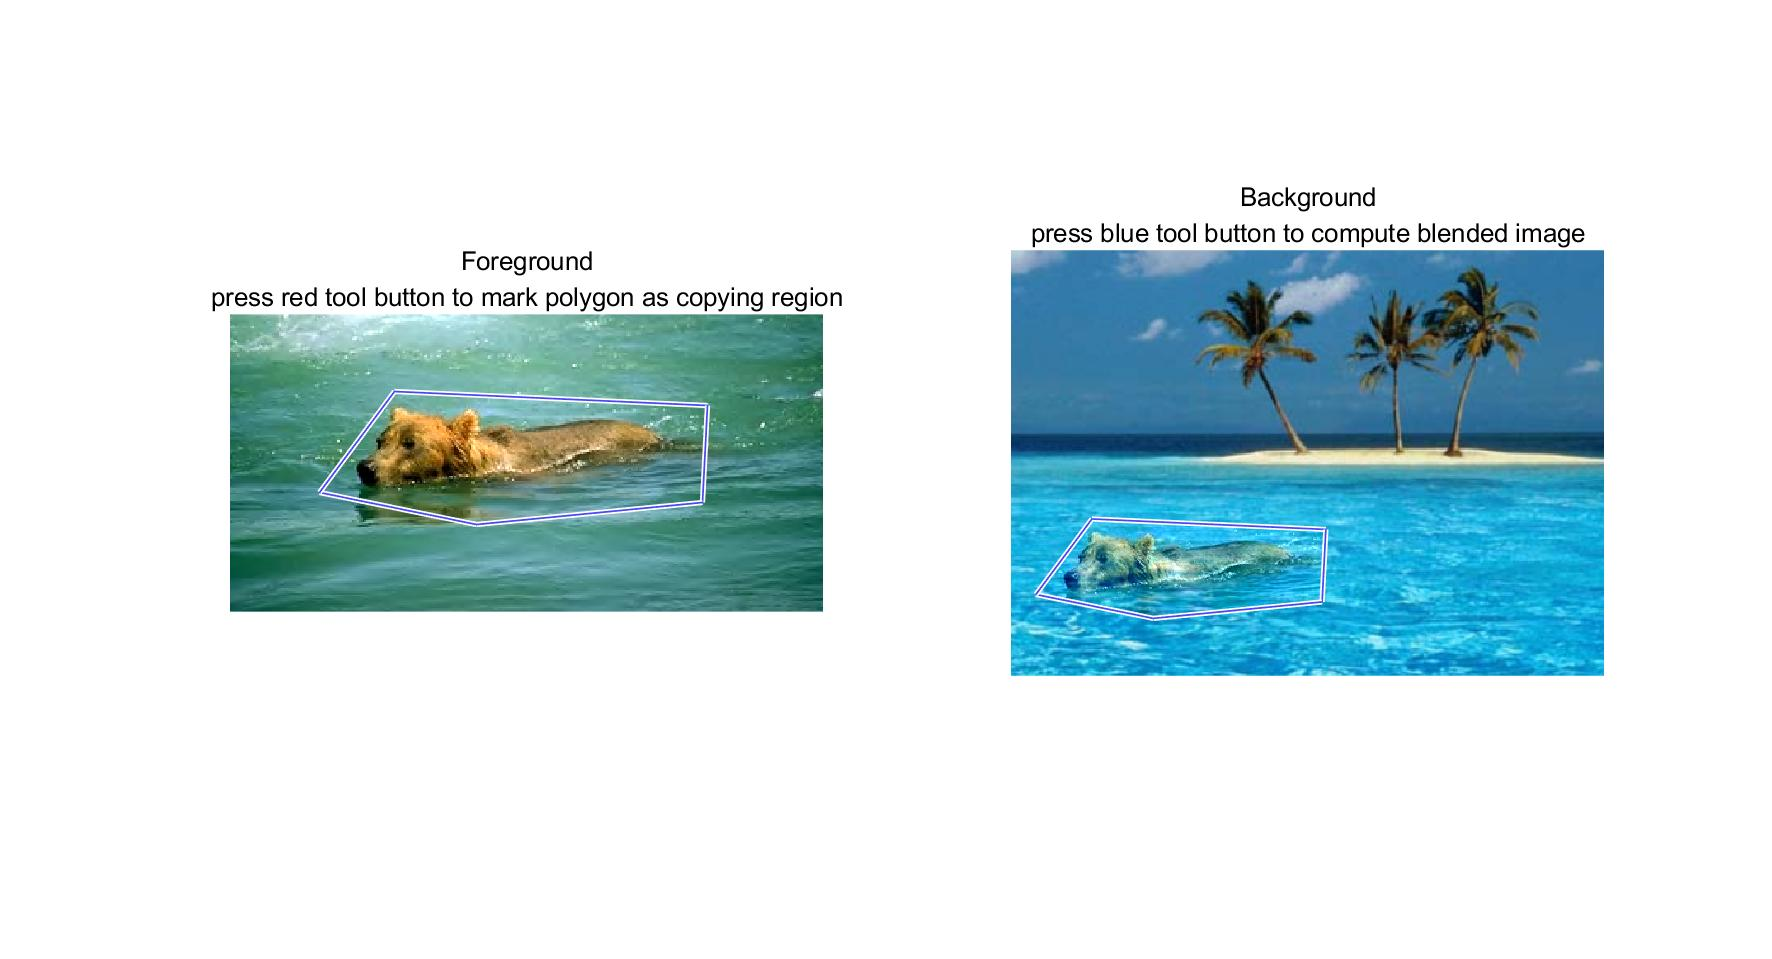
\includegraphics[width=1.0\textwidth]{fig1.jpg}
  \caption{BearInWater}
  \label{fig:fig-1}
\end{figure}

\begin{figure}[htb]
  \centering
  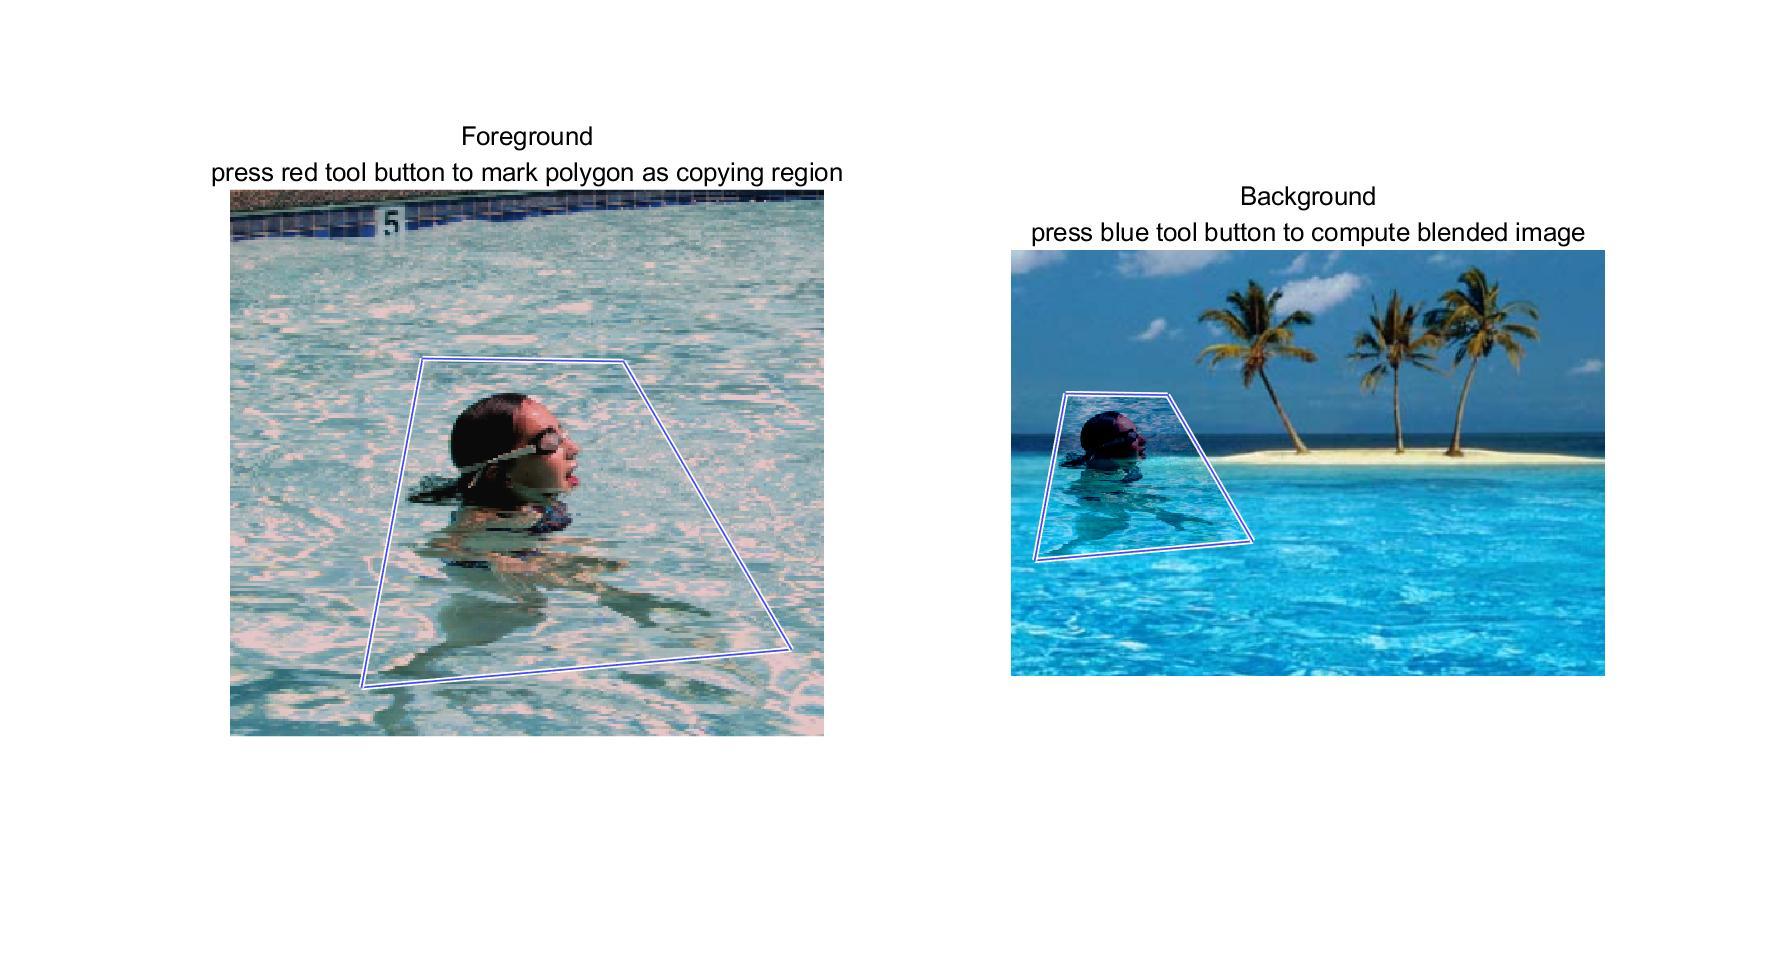
\includegraphics[width=1.0\textwidth]{fig3.jpg}
  \caption{GirlInWater}
  \label{fig:fig-1}
\end{figure}

\newpage
程序实现了多边形区域选取物体图片,拖动新背景图片中的对应多边形实时将物体融入新背景,拖动过程中图片变换较流畅。这里我们分别选取狗和人的图片将其放入海洋图片中,可以看出物体融入效果较好。


















\end{document}
